\documentclass{article}
\usepackage[utf8]{inputenc}
\usepackage[english]{babel}
\usepackage[ddmmyyyy]{datetime}
\usepackage{svg}
\usepackage[a4paper, total={6in, 10in}]{geometry}
%\usepackage{graphicx}
\usepackage[utf8]{inputenc}
\usepackage{hyperref}
\usepackage{comment}
%\usepackage{tikz}
%\usepackage{subcaption}
\usepackage{amssymb}
\usepackage{amsmath}
\usepackage{gensymb}
\usepackage[english]{babel}
\usepackage{csquotes}
\usepackage[backend=biber,style=numeric,citestyle=chem-acs]{biblatex}
\addbibresource{references.bib}


\title{Thermophilic GH5\_7 project}
\author{Simon Birgersson}
\date{\today}
\def\signed #1 (#2){{\unskip\nobreak\hfil\penalty50
  \hskip2em\hbox{}\nobreak\hfil\sl#1\/ \rm(#2)
  \parfillskip=0pt \finalhyphendemerits=0 \par}}


\newdateformat{mydate}{\twodigit{\THEDAY}{ }\shortmonthname[\THEMONTH], \THEYEAR}
\makeatletter
\def\@maketitle{   % custom maketitle
\noindent {\Large \bfseries \color{black} \@title}  \\ \hrule \noindent  \\ \@author \\ \@date
}


\begin{document}
\maketitle

\section{Introduction}
Glycoside Hydrolases can be used for production of novel glyconjugates usng transglycosylation reactions. This is of interest in utilizing waste streams in bioconversion of wood material, such as lignocellulose, which is underutilized in current industrial settings. Instead this material stream can be used to produce novel materials and platform chemicals only accessible through petrochemical sources in the past. With this in mind, I've set out to assess the potential of some Thermophilic GH:s for use in these reactions, as the thermostability is potentially helpful in industrial application. I'm also investiated the possibility of the structure of these enzymes is conducive to increased stability in organic solvents at lower temperature, besides being more stable at higher temperatures. The enzymes I will be utlizing are TpMan5A, from \textit{Thermotoga petrophila} and BpMan5A, from \textit{Bacillus pumilus}. These are described previously in literature, and will be discussed briefly in the sections Below:

\subsection{TpMan5A}
\textit{T. petrophila} is a hyperthermophillic, Gram-negative bacterium from the Kubiki oil resevoir in Niigata (Japan), and its enzymes show good promise for biotech application. Some work has already been done on TpMan5A, described below:
\begin{itemize}
  \item Santos et al \cite{Santos2010} describes how the crystal structure (PDB: 1QNR) was generated. There are two crystals, each from two separate crystallization procedure (is this the reason for the rotamers in 1QNR?).

  \item dos Santos et. al \cite{DosSantos2012} describes how the stability is affected in different deletion mutants, thus elucidating stabilizing elements in the structure. They also carried out a central composite experimental design in order to find optimal pH and temperature values, results of which is included in table \ref{tab:temp_pH_opt}. In summary, they determined that the $\Delta$CBM mutant showed no significant change in substrate specificity or catalytic effiency, but showed much worse thermal stability ($\Delta T_{melt}=100-88$).

    \item da Silva et al. \cite{DaSilva2020} attempts to characterize TpMan5A through structural analysis and some DLS studies of thermostability. They found out that the second immunoglobulin-like domain acts as a thermostabilizing domain and allows the enzyme to act even under hyperthermal conditions.
\end{itemize}

\subsection{BpMan5A}
BpMan5A is a GH5 endo-1,4-$\beta$-mannosidase from \textit{B. pumilus}. \textit{B. pumilus} is a Gram-positive, aerobic, spore-forming bacterium commonly found in the \textit{rhizosphere}, the area close to plant roots directly under the influence of plant secretions etc. \textit{B. pumilus} is non-pathogenic an highly resistant to environmental stress. The specific strain collected in Zang et al \cite{Zang2015} is collected from Tibet and has shown good ability in decomposing lignocellulosic plant mass.

\begin{itemize}
  \item Zang et al. \cite{Zang2015} identified BpMan5A as a mannanase, expressed, purified, and finally characterized it. pH optimum, pH activity, temperature optimum, and temperature stability (figure: \ref{fig:zang}). Its products are mainly M2, M3, M5 when utlizing Locust Bean Gum (LBG) as substrate.

 \begin{figure}[!h]
	\centering
	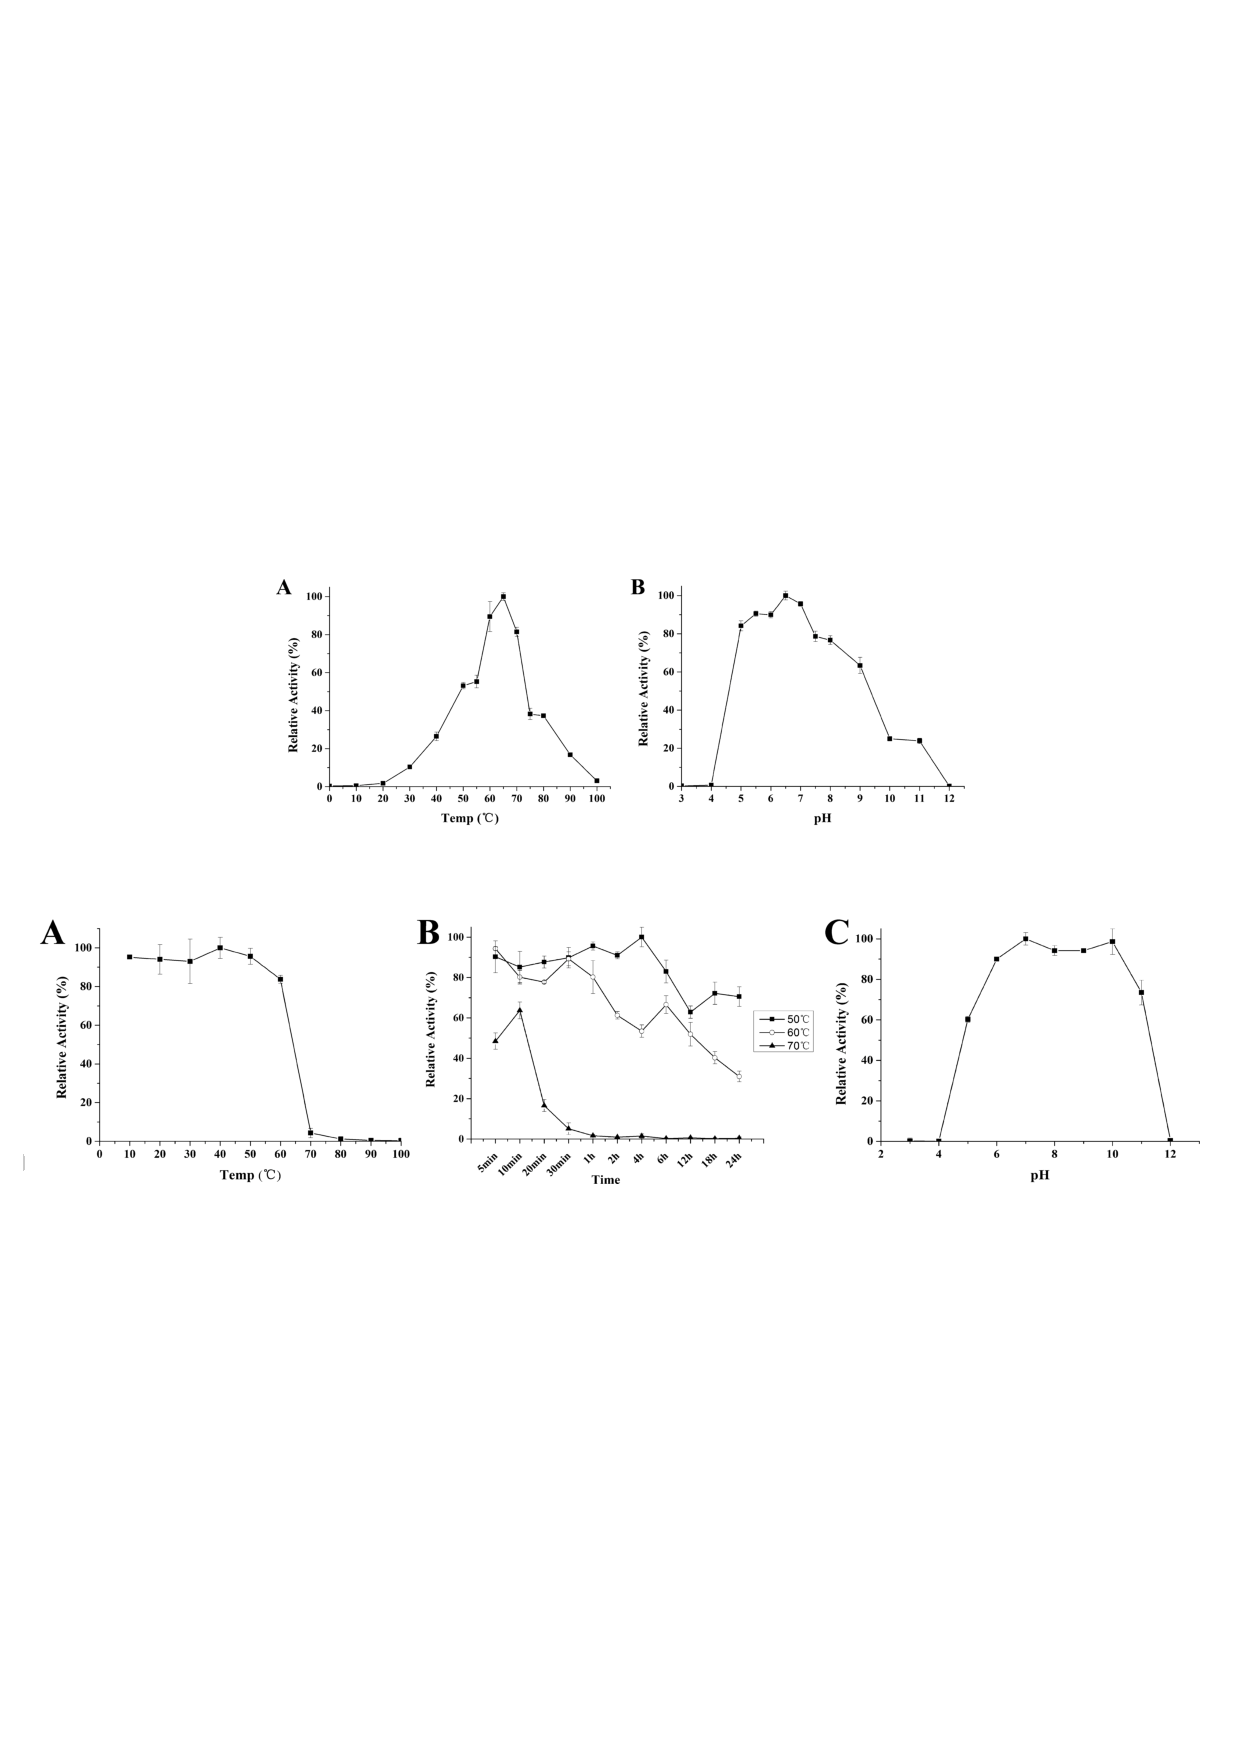
\includegraphics[width=0.95\textwidth]{figures/Zang.pdf}
	\caption{Shows some parameters characterized in Zang et al \cite{Zang2015}}
	\label{fig:zang}
\end{figure}
\end{itemize} % Zang figure

\section{Activity Measurement / Basic Characterization}
The goal for me was to map out how the activity and stability of TpMan5A and BpMan5A were affected by temperature, pH, and the presence of various acceptor solutions in order to determine proper reaction parameters for maximizing glyconjugate production yield. Some of these values were available in literature, and will be presented in table \ref{tab:temp_pH_opt}:

\begin{table}[ht]
\centering
  \begin{tabular}{llll}
  \hline
    parameter: & TpMan5A              & BpMan5A              & source: \\
    \hline
    $T_{opt}$    & 65$\celsius$             & 65$\celsius$ C          &  \\
    $T_{stab}$   & \>90$\degree$ C for 24h & $\<$30min 70$\celsius$ C  &  \\
    $pH_{opt}$   &  6.5                    & 6.5                    &  \\
    $pH_{stab}$  & 6$\rightarrow$10        & inactive at pH 3       &  \\
    \hline
  \end{tabular}
  \caption{Shows some optimal temp and pH for TpMan5A and BpMan5A, gathered on my own or supplied from literature.}
  \label{tab:temp_pH_opt}
\end{table} % lit. parameter table


\begin{figure}[h]
    \centering
    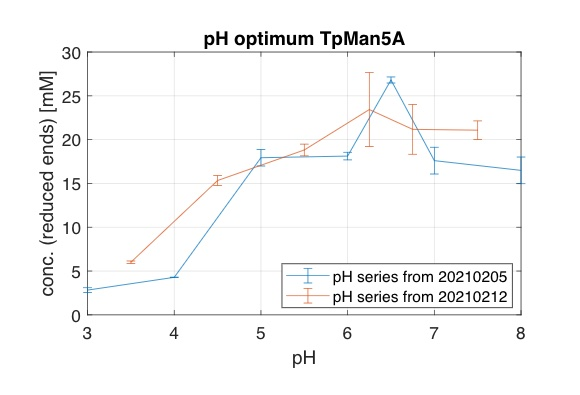
\includegraphics[width=0.5\textwidth]{figures/pH_optimum.jpg}
    \caption{shows results of pH-resolved DNS assay of TpMan5A performed 20210212}
    \label{fig:pH-optimum}
\end{figure} % pH optimum graph

\section{Acceptor Screening}

\section{Future Project Plans}
Transfer reaction (MS)
HPAEC reaction (end point assay)

\newpage
\printbibliography

\end{document}
